\chapter{Krav til specifikt bevægelsesmønster} \label{Monster}
Kravet om et specifkt bevægelsesmønster er lavet for at sikre, at hele brystet bliver scannet af Ultralydsscanner. Ved traditionelle scanninger, foretaget af radiologer, føres ultralydsproben i en sinus-lignende kurve med overlap, startende fra højre side af højre bryst til venstre side af højre bryst, og derefter fra højre side af venstre bryst ud til venstre side af venstre bryst. Det skal sikres, at ultralydsproben starter og slutter uden for brystvævet, hvilket sikrer, at hele brystet er scannet. Bevægelsesmønsteret er illustreret i Figur \ref{Probensbevagelse} nedenfor. 

\begin{figure}[H]
    \centering
    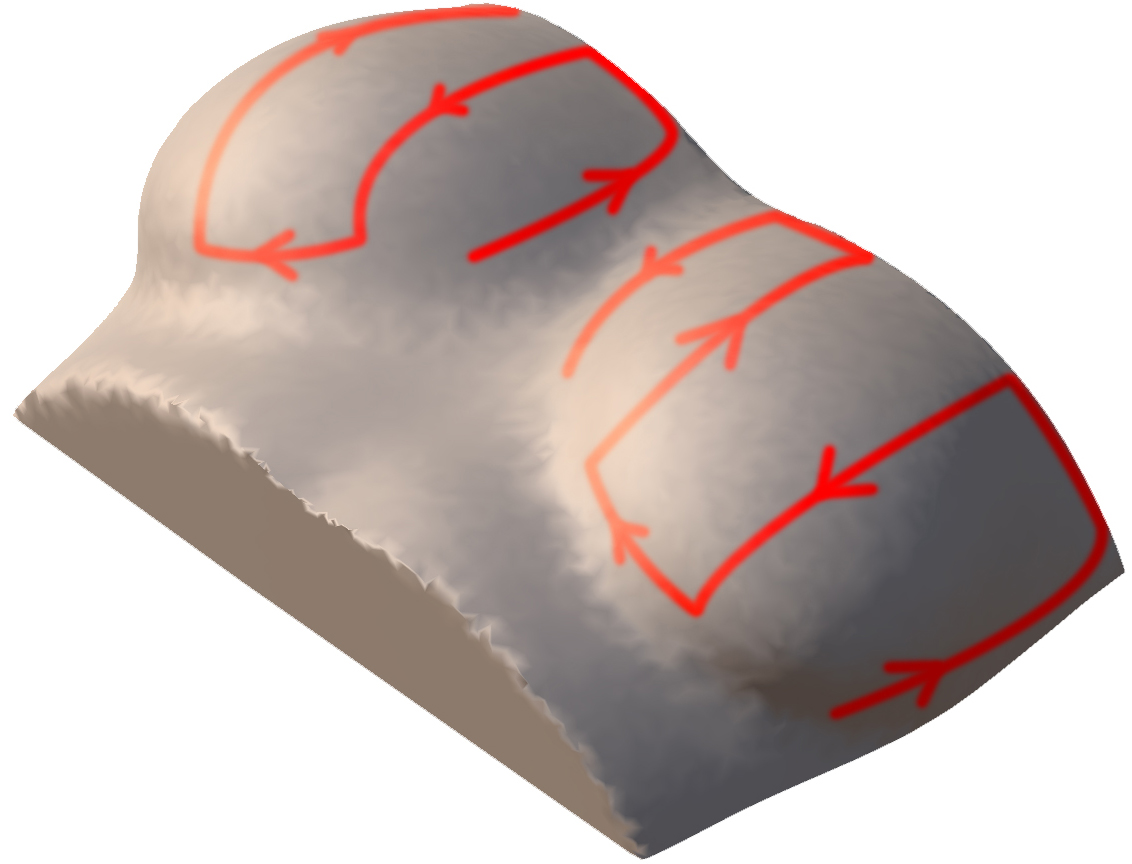
\includegraphics[width=0.75\textwidth]{figurer/d/probebevagelse}
    \caption{Probens bevægelsesbane på brystet}
    \label{Probensbevagelse}
\end{figure}

Bevægelsesmønsteret er bestemt ud fra interview med radiolog Lars Bolvig. For interview se bilag \ref{Telefoninterview}. 